\documentclass[tikz,border = 10pt]{standalone}

\begin{document}
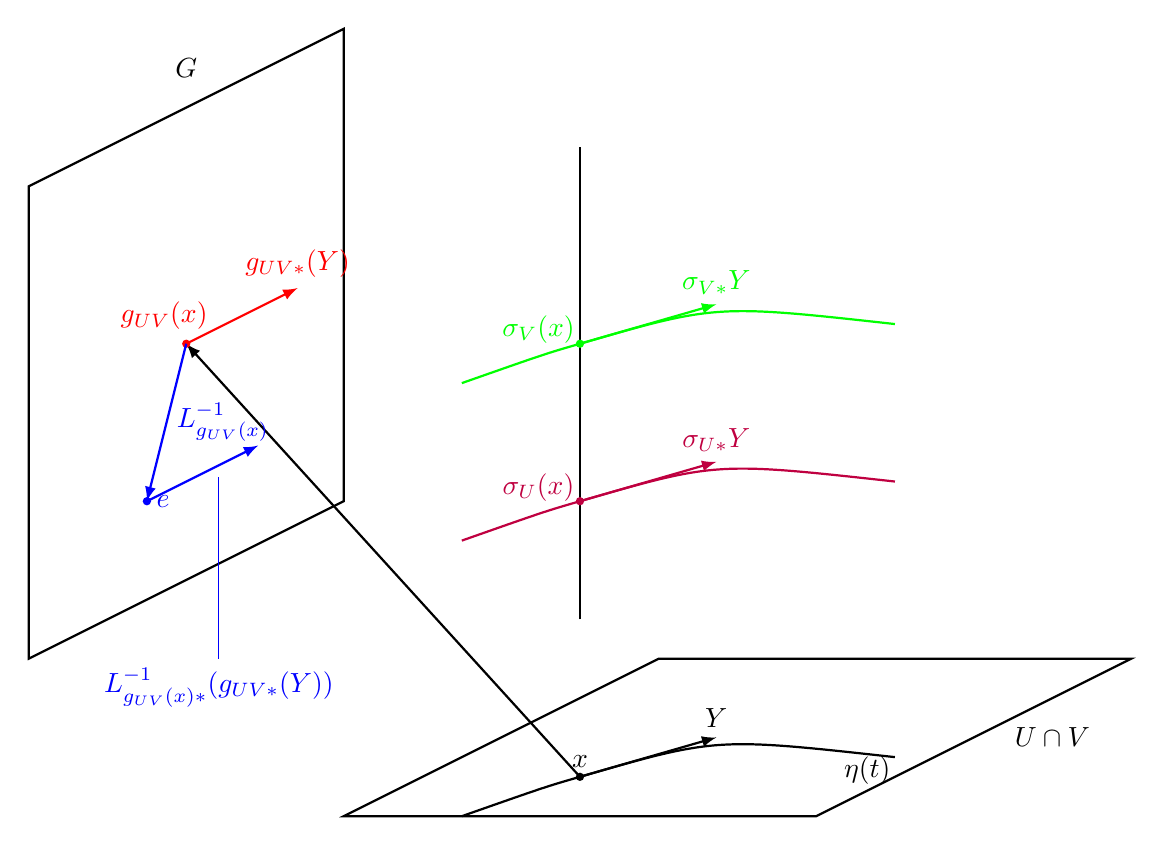
\begin{tikzpicture}
  \node at (-4,7.5) {$G$};
  \draw[thick] (-6,0) -- (-2,2) -- (-2,8) -- (-6,6) -- cycle;
  \node at (7,-1) {$U \cap V$};
  \draw[thick] (-2,-2) -- (2,0) -- (8,0) -- (4,-2) -- cycle;
  \draw[thick,-latex] (1,-1.5) -- ({1+2 * cos(30)},{ -1.5 + 1 * sin(30)});
  \node[above] at ({1+2 * cos(30)},{ -1.5 + 1 * sin(30)}) {$Y$};
  \draw[thick] (-0.5,-2)..controls({1-0.5 * cos(30)},{-1.5-0.25*sin(30)}).. (1,-1.5)..controls ({1+2 * cos(30)},{ -1.5 + 1 * sin{30}}) .. (5,-1.25);
  \fill  (1,-1.5) circle(1.5pt) node[above]{$x$}; 

  \draw[thick, -latex] (1,-1.5) --(-4,4);

  \fill[red] (-4,4) circle(1.5pt) node[xshift = -8,yshift =10]{$g_{UV}(x)$};
  \draw[thick,-latex,red] (-4,4) -- ({-4+ 2*cos(45)} , {4 + 1 *sin(45)}) node[above]{$g_{UV*}(Y)$};
  \fill[blue](-4.5,2) circle (1.5pt) node[right]{$e$};
  \draw[thick,-latex,blue](-4,4) -- (-4.5,2) node[pos = 0.5,right]{$L_{g_{UV}(x)}^{-1}$};
  \draw[thick,-latex,blue] (-4.5,2) -- ({-4.5+ 2*cos(45)} , {2 + 1 *sin(45)});
  \draw[fill = white,blue]({-5+ 2*cos(45)} , {1.6 + 1 *sin(45)}) -- ({-5+ 2*cos(45)},0) node[below,pos = 1]{$L^{-1}_{g_{UV}(x)*}(g_{UV*}(Y))$};

  \node[yshift = -5, xshift = -10] at (5,-1.25) {$\eta(t)$};

  \draw[thick] (1,0.5) -- (1,6.5);
  \draw[thick,green] (-0.5,3.5)..controls({1-0.5 * cos(30)},{4-0.25*sin(30)}).. (1,4)..controls ({1+2 * cos(30)},{ 4 + 1 * sin{30}}) .. (5,4.25);
  \draw[thick,-latex,green] (1,4) -- ({1+2 * cos(30)},{ 4 + 1 * sin(30)}) node[pos = 1,above]{$\sigma_{V*}Y$};
  \fill[green] (1,4) circle(1.5pt) node[xshift = -15,yshift = 5]{$\sigma_V(x)$};

  \draw[thick,purple] (-0.5,1.5)..controls({1-0.5 * cos(30)},{2-0.25*sin(30)}).. (1,2)..controls ({1+2 * cos(30)},{ 2 + 1 * sin{30}}) .. (5,2.25);
  \draw[thick,-latex,purple] (1,2) -- ({1+2 * cos(30)},{ 2 + 1 * sin(30)}) node[pos = 1,above]{$\sigma_{U*}Y$};
  \fill[purple] (1,2) circle(1.5pt) node[xshift = -15,yshift = 5]{$\sigma_U(x)$};

  \end{tikzpicture}
\end{document} 
